\documentclass[12pt,openright,oneside,a4paper,english,brazil]{abntex2}

% Pacotes básicos 
\usepackage{lmodern}			% Usa a fonte Latin Modern		
\usepackage[defaultsans,scale=0.9]{lato}
\usepackage[T1]{fontenc}		% Selecao de codigos de fonte.
\usepackage[utf8]{inputenc}		% Codificacao do documento (conversão automática dos acentos)
\usepackage{lastpage}			% Usado pela Ficha catalográfica
\usepackage{indentfirst}		% Indenta o primeiro parágrafo de cada seção.
\usepackage{color}				% Controle das cores
\usepackage{graphicx}			% Inclusão de gráficos
\usepackage{float}
\usepackage{microtype} 			% para melhorias de justificação
\usepackage{amsmath}
\usepackage{amsfonts}
\usepackage{subcaption}

\renewcommand\thesubsubsection{}
\DeclareMathOperator*{\argmax}{arg\,max}
\DeclareMathOperator*{\argmin}{arg\,min}


% CONFIGURAÇÕES DE PACOTES

% Informações de dados para CAPA e FOLHA DE ROSTO
\titulo{	Restauração de Imagens de Placas de Veículos Usando Super-resolução}
\autor{David Campos Anchieta}
\local{Belém - PA}
\data{2018}
\orientador{Prof. Dr. Ronaldo de Freitas Zampolo}
\instituicao{%
	Universidade Federal do Pará
	\par
	Instituto de Tecnologia
	\par
	Faculdade de Engenharia da computação e Telecomunicações}
\tipotrabalho{Trabalho de Conclusão de Curso}
% O preambulo deve conter o tipo do trabalho, o objetivo, 
% o nome da instituição e a área de concentração 

% ISSUE: redigir preambulo
\preambulo{ Trabalho de conclusão de curso apresentado à Faculdade de Engenharia da Computação e Telecomunicações da Universidade Federal do Pará como requisito parcial para a obtenção de grau de Bacharel em Engenharia da Computação. }


% Configurações de aparência do PDF final

% alterando o aspecto da cor azul
\definecolor{blue}{RGB}{41,5,195}

% informações do PDF
\makeatletter
\hypersetup{
			%pagebackref=true,
		pdftitle={\@title}, 
		pdfauthor={\@author},
			pdfsubject={\imprimirpreambulo},
			pdfcreator={LaTeX with abnTeX2},
		pdfkeywords={abnt}{latex}{abntex}{abntex2}{trabalho acadêmico}, 
		colorlinks=true,       		% false: boxed links; true: colored links
			linkcolor=blue,          	% color of internal links
			citecolor=blue,        		% color of links to bibliography
			filecolor=magenta,      		% color of file links
		urlcolor=blue,
		bookmarksdepth=4
}
\makeatother

% Espaçamentos entre linhas e parágrafos 
% O tamanho do parágrafo é dado por:
\setlength{\parindent}{1.3cm}

% Controle do espaçamento entre um parágrafo e outro:
\setlength{\parskip}{0.2cm}  % tente também \onelineskip

% compila o indice
\makeindex

% Início do documento
\begin{document}

% Seleciona o idioma do documento (conforme pacotes do babel)
%\selectlanguage{english}
\selectlanguage{brazil}

% Retira espaço extra obsoleto entre as frases.
\frenchspacing 
% ELEMENTOS PRÉ-TEXTUAIS

% Capa
\imprimircapa

% Folha de rosto
\imprimirfolhaderosto

% Inserir folha de aprovação

% Isto é um exemplo de Folha de aprovação, elemento obrigatório da NBR
% 14724/2011 (seção 4.2.1.3). Você pode utilizar este modelo até a aprovação
% do trabalho. Após isso, substitua todo o conteúdo deste arquivo por uma
% imagem da página assinada pela banca com o comando abaixo:
%
% \includepdf{folhadeaprovacao_final.pdf}
%

\begin{folhadeaprovacao}
%ISSUE: folha de aprovação
	\begin{center}
		{\ABNTEXchapterfont\large\imprimirautor}

		\vspace*{\fill}\vspace*{\fill}
		\begin{center}
			\ABNTEXchapterfont\bfseries\Large\imprimirtitulo
		\end{center}
		\vspace*{\fill}
		
		\hspace{.45\textwidth}
		\begin{minipage}{.5\textwidth}
				\imprimirpreambulo
		\end{minipage}%
		\vspace*{\fill}
	 \end{center}
				
	 Trabalho aprovado. \imprimirlocal, 09 de fevereiro de 2018:
% ISSUE: Data da folha de aprovação

	 \assinatura{\textbf{\imprimirorientador} \\ Orientador} 
	 \assinatura{\textbf{Professor} \\ Convidado 1}
	 \assinatura{\textbf{Professor} \\ Convidado 2}
	 %\assinatura{\textbf{Professor} \\ Convidado 3}
	 %\assinatura{\textbf{Professor} \\ Convidado 4}
% ISSUE: Nomes dos integrantes da banca

	 \begin{center}
		\vspace*{0.5cm}
		{\large\imprimirlocal}
		\par
		{\large\imprimirdata}
		\vspace*{1cm}
	\end{center}
	
\end{folhadeaprovacao}

% Dedicatória
%\begin{dedicatoria}
%ISSUE: dedicatória
	 %\vspace*{\fill}
	 %\centering
	 %\noindent
	 %\textit{ DEDICATÓRIA} \vspace*{\fill}
%\end{dedicatoria}

% Agradecimentos
%\begin{agradecimentos}
%ISSUE: agradecimentos


%\end{agradecimentos}

% Epígrafe
\begin{epigrafe}
%ISSUE: epígrafe
		\vspace*{\fill}
	\begin{flushright}
		\textit{Além disso, filho meu, sê avisado. \\
		De fazer muitos livros não há fim; \\
		e o muito estudar é enfado da carne. \\
Eclesiastes 12:12
		}
	\end{flushright}
\end{epigrafe}

% RESUMOS

% resumo em português
\setlength{\absparsep}{18pt} % ajusta o espaçamento dos parágrafos do resumo
\begin{resumo}
%ISSUE: resumo pt
	Esta monografia relata a teoria, implementação e resultados da aplicação de um Método de Super-resolução Bayesiana na restauração de imagens de placas de veículos.
	Ao longo do texto são discutidos um breve histórico das técnicas de restauração de imagens, o modelo de observação mais utilizado pelos métodos de Super-resolução, um apanhado dos principais métodos de Super-resolução.
	Este trabalho apresenta uma descrição detalhada do método de Super-resolução Bayesiana proposto pro Michael Tipping e Christopher Bishop.
	A implementação do método é descrita junto com os resultados.

 \textbf{Palavras-chave}: Super-resolução, restauração de imagens, inferência Bayesiana.
\end{resumo}

% resumo em inglês
\begin{resumo}[Abstract]
%ISSUE: resumo en
 \begin{otherlanguage*}{english}
	This work reports on the theory, implementation and results of the application of a Bayesian Super-resolution Method in vehicle license plate image restoration.
	Throughout the text a brief history of image restoration techniques is presented, the observation model most used by Super-resolution methods is decribed and a collection of the main methods of Super-resolution are summarized.
	This paper presents a detailed description of the Bayesian Super-resolution method proposed by Michael Tipping and Christopher Bishop.
	An implementation of the method is described in conjunction with the results.
	\vspace{\onelineskip}
	\noindent 
 \textbf{Keywords}: Super-resolution, image restoration, Bayesian inference.
 \end{otherlanguage*}
\end{resumo}


% inserir lista de ilustrações
\pdfbookmark[0]{\listfigurename}{lof}
\listoffigures*
\cleardoublepage
% ---

% ---
% inserir lista de tabelas
% ---
%\pdfbookmark[0]{\listtablename}{lot}
%\listoftables*
%\cleardoublepage
% ---

% ---
% inserir lista de abreviaturas e siglas
% ---
\begin{siglas}
	\item[SR] Super-resolução
	\item[HR] \emph{High resolution}
	\item[LR] \emph{Low resolution}
	\item[PDF] \emph{Probalility density function}
	\item[IBP] \emph{Iterative Back Projections}

\end{siglas}
% ---

% ---
% inserir lista de símbolos
% ---
\begin{simbolos}
%ISSUE: lista de símbolos
	\item[$ \mathbf{x} $] Vetor com os dados da imagem de alta resolução.
	\item[$ \mathbf{y}_k $] Vetor da imagem de alta resolução de número k.
	\item[$ K $] Número de imagens de baixa resolução.
	\item[$ N $] Número de pontos na imagem de alta resolução.
    \item[$ M $] Número de pontos na imagem de baixa resolução.
    \item[$ \mathbf{W}^{(k)}$] Matriz de degradação da imagem de número k.
    \item[$ \gamma $] Largura da função de espalhamento de ponto.
    \item[$ \theta_k $] Ângulo de rotação da imagem de número k.
    \item[$ \mathbf{s}_k $] Vetor com deslocamento bidimensional da imagem de baixa resolução de número k.
    \item[$ \mathbf{Z}_x $] Matriz de covariância da distribuição a priori de $\mathbf{x}$.
    \item[$ \mathbf{\Sigma}$] Matriz de covariância da distibuição a posteriori de $\mathbf{x}$ condicionada aos parâmetros de degradação e conjunto de todos os $\mathbf{y}^{(k)}$.
    \item[$ \boldsymbol{\mu} $] Vetor média da distibuição a posteriori de $\mathbf{x}$ condicionada aos parâmetros de degradação e conjunto de todos os $\mathbf{y}^{(k)}$.
    \item[$ \beta $] Inverso da variância do ruído.
    \item[$ | \cdot | $] Determinante de matriz.
    \item[$\| \cdot \|$] Norma de um vetor.
    
\end{simbolos}
% ---

% ---
% inserir o sumario
% ---
\pdfbookmark[0]{\contentsname}{toc}
\tableofcontents*
\cleardoublepage
% ---



% ----------------------------------------------------------
% ELEMENTOS TEXTUAIS
% ----------------------------------------------------------
\textual

% ----------------------------------------------------------
% Introdução (exemplo de capítulo sem numeração, mas presente no Sumário)
% ----------------------------------------------------------
\chapter[Introdução]{Introdução}
% \addcontentsline{toc}{chapter}{Introdução}
% ----------------------------------------------------------
%ISSUE: introdução
%ISSUE: Corrigir a capitalização de seção
%ISSUE: Corrigir a capitalização de capítulo
%ISSUE: Corrigir a capitalização de figura 
%ISSUE: Corrigir a capitalização de tabela
%ISSUE: Corrigir a capitalização de equação

% CONTEXTUALIZAÇÃO: ONDE MEU PROBLEMA APARECE?
A disponibilidade de imagens de alta resolução é uma vantagem para a execução de qualquer trabalho que envolva a captação e interpretação de informações através de imagens digitais.
Como exemplo disso podemos citar as imagens médicas, nas quais quanto melhor a
qualidade da imagem, mais fácil é diferenciar as estruturas retratadas com o objetivo
de diagnosticar doenças.
Também há o caso dos sistemas de vigilância, nos quais quanto melhor a resolução espacial
da imagem, mais viável se torna a identificação de veículos e criminosos.

% DELIMITAÇÃO: QUE PROBLEMA ESTOU RESOLVENDO?
Hoje em dia, com as frequentes ameaças à segurança das pessoas em diversos lugares do mundo, os cidadãos sentem a necessidade de investir na própria segurança privada para proteger a si mesmos e seus patrimônios.
Por causa dessa necessidade, houve uma popularização de sistemas de vigilância monitoramento.
As câmeras de segurança já são tão onipresentes em grandes cidades que é praticamente impossível que um cidadão comum saia à rua e não tenha a sua imagem gravada por pelo menos uma delas.

No entanto, apesar da presença geral dos sistemas de vigilância, a maioria dos equipamentos utilizados é de baixa qualidade, o que se reflete nas imagens captadas por eles.
A consequência disso é que muitas vezes as câmeras de monitoramento registram cenas de crimes,
mas as imagens deterioradas nem sempre ajudam a trazer à luz informações importantes, como o rosto de um criminoso ou a placa de um carro, por exemplo.

Não obstante, mesmo com necessidade evidente de se melhorar a qualidade das imagens geradas por sistemas de vigilância,
também há o dilema constante entre aumentar a qualidade das imagens registradas e o custo de implementar manter o sistema de monitoramento funcionando.
Quanto melhor a qualidade da imagem, maior é o custo do equipamento e mais capacidade de armazenamento será necessária para guardar uma quantidade útil de todas as imagens gravadas.


% SOLUÇÕES: O QUE JÁ EXISTE QUE RESOLVE ESTE PROBLEMA?
Face ao dilema das imagens geradas por sistemas de vigilância,
a melhor solução a curto prazo seria aprimorar as imagens que estão sendo geradas pelas câmeras de monitoramento que já temos hoje.
Esse aprimoramento seria feito através de restauração de imagens digitais.

A demanda pelo desenvolvimento de técnicas de restauração de imagens ganhou força no fim da década de 1950, quando a sua principal aplicação era na área de imagens astronômicas.
Naquele contexto, era necessário restaurar as primeiras imagens recebidas de sondas e satélites artificiais.
As imagens captadas por sondas espaciais e satélites artificiais sofriam degradações próprias do ambiente onde esses objetos trabalhavam.

Após tantos anos, a restauração de imagens digitais continua tendo sua importância na astronomia, mas também é uma ferramenta para outras áreas como medicina, mídia e ciências forenses \cite{banham1997digital}.
Cada uma com suas particularidades e necessidades.

% SOLUÇÃO ESCOLHIDA: O QUE ELA É E COMO FUNCIONA?
Este trabalho descreve a implementação e teste de um método de restauração de imagens de placas de veículos usando super-resolução bayesiana.
O método utilizado foi apresentado por Michael Tipping e Christopher Bishop \cite{tipping2003bayesian}.
Em resumo, o algorítimo apresentado define um modelo de observação no qual as degradações sofridas pela imagem durante o processo de aquisição são parametrizadas.
Então são usadas inferências bayesianas para estimar os parâmetros de degradação a partir das imagens de baixa resolução, para então estimar a imagem de alta resolução a partir destes parâmetros.

% VANTAGENS: POR QUE ESTA SOLUÇÃO E NÃO AS OUTRAS?
Esta solução foi escolhida devido à adequação do algorítimo à aplicação desejada, que é a restauração de uma imagem de placa de veículo a partir de várias imagens degradadas.
A ideia principal é que o método posa ser usado para revelar os caracteres de uma placa de um veículo que tenha sido captado por uma câmera de vídeo, mas que não esteja visível devido à má qualidade da imagem.

Também vale destacar a relativa simplicidade de implementação do método escolhido, o qual também possibilita ajustes afim de reduzir seu custo computacional.

% ESTRUTURA: O QUE TEM NOS CAPÍTULOS SEGUINTES?
% ISSUE: Escrever estrutura do trabalho

Esta monografia está organizada da seguinte forma: O Capítulo \ref{chap:superRes} apresenta o conceito de Super-resolução e descreve resumidamente as principais técnicas.
O Capítulo \ref{chap:srbayes} apresenta e descreve com detalhes o método de Super Resolução Bayesiana, o qual é objeto de estudo deste trabalho.
O Capítulo \ref{chap:resultados} descreve o contexto no qual o método foi testado e apresenta os resultados das simulações.
As considerações finais acerca do trabalho são feitas no Capítulo \ref{chap:conclusao}.


\chapter{Restauração de Imagens Usando Super-resolução}
\section{Introdução}
Entende-se por Super-resolução o processo de obtenção de uma ou mais imagens de alta resolução a partir de uma ou mais imagens de baixa resolução.
Técnicas de super-resolução são pesquisadas desde os anos 1970 e têm despertado um grande interesse de estudo nas últimas décadas.
As aplicações de técnicas de SR são diversas e incluem aprimoramentos de imagens médicas, de imagens de rosto, de texto e impressões digitais \cite{nasrollahi2014super}.

Vale esclarecer que, neste trabalho, a palavra \textit{resolução} se refere à resolução espacial de uma imagem, a qual mede a densidade de pontos por unidade de área em uma imagem \cite{zibetti2007super}.

Este capítulo fará uma breve síntese do histórico das técnicas de super-resolução e seus principais exemplares.

\section{Modelo de Observação}
\label{sec:obsmodel}

Definir um modelo de observação que relacione a imagem de alta resolução às imagens de baixa resolução observadas é fundamental para o desenvolvimento de qualquer técnica de super-resolução.

O modelo de observação deste trabalho simula cinco tipos de alteração aplicadas por sistemas de aquisição de imagens, a saber: rotação, deslocamento, espalhamento de ponto, subamostragem e ruído.
Este modelo de observação é descrito tanto em \cite{tipping2003bayesian} quanto em outros trabalhos relacionados \cite{pickup2007bayesian, Capel01a}.

As alterações de deslocamento linear e rotação tentam simular um possível movimento aleatório da câmera em relação ao objeto.
A transformação de espalhamento de ponto simula um efeito de desfoque causado por um possível desajuste nos aspectos ópticos da câmera.
A subamostragem representa a perda de resolução espacial aplicada à imagem captada por um sensor CMOS ou CCD, por exemplo.
que seria menor do que a necessária para registrar os dados da imagem acima da taxa de Nyquist.

Pela conveniência do modelo de observação, a imagem de alta resolução de dimensões $m \times n$ é representada por um vetor coluna $\mathbf{x} = [x_1, x_2, ... , x_{N-1}, x_N]^T$ onde $N ={} m \times n$. Ou seja, os valores dos pixels da imagem são rearranjados em um vetor de comprimento $N$.

Sabendo disso, a relação entre uma imagem de alta resolução $\mathbf{x}$ e uma imagem degradada $\mathbf{y}^{(k)}$ é resumida em (\ref{eq:degradation}). Onde $k = 1,2,...,K$; sendo $K$ o número total de quadros obtidos a partir da cena de alta resolução $\mathbf{x}$.

\begin{equation}
	\label{eq:degradation}
	\mathbf{y}^{(k)} = \mathbf{W}^{(k)}\mathbf{x} + \mathbf{n}^{(k)}
\end{equation}

O ruído, representado por $\mathbf{n}$ é um vetor de variáveis aleatórias Gaussianas independentes de média zero e variância $1/\beta$.

A matriz de sistema $\mathbf{W}$ aplica as transformações de rotação, deslocamento, subamostragem e espalhamento de ponto ao ser multiplicada pela imagem de alta resolução $\mathbf{x}$.
Pelas propriedades da multiplicação de matrizes, é natural que as dimensões da matriz do sistema sejam $M \times N$; onde $M$ é o número de pixels da imagem resultante.
Também se espera que $N \gg M$.

A matriz $\mathbf{W}$ depende de três parâmetros de transformação: a largura da função de espalhamento de ponto $\gamma$, um ângulo de rotação $\theta$ e um vetor de deslocamento linear $\mathbf{s}$.
Os elementos da matriz são dados por (\ref{eq:wmatrix}) com a função de espalhamento de ponto descrita em (\ref{eq:psf}) enquanto os parágrafos seguintes demonstram como as demais transformações são incorporadas à matriz de sistema.

\begin{gather}
	\label{eq:wmatrix}
	W^{(k)}_{ji} = \widetilde{W}^{(k)}_{ji} / \sum_{i'} \widetilde{W}^{(k)}_{ji} \\
	\label{eq:psf}
	\widetilde{W}^{(k)}_{ji} = \exp \left\{- \frac{\|\mathbf{v}_i - \mathbf{u}^{(k)}_j\|^2}{\gamma^2} \right\}
\end{gather}

Os vetores $\mathbf{u}^{(k)}_j$ representam o centro da função de espalhamento de ponto e é descrito em (\ref{eq:psfcenter}).
Caso não houvesse espalhamento de ponto, as coordenadas $\{\mathbf{u}_1, \mathbf{u}_2,\mathbf{u}_3,..., \mathbf{u}_M\}$ seriam os pontos de amostragem da imagem de baixa resolução na imagem de alta resolução.
A Figura \ref{fig:transformations} mostra como se dá o processo de subamostragem e outras transformações bidimensionais.

O efeito da transformação de espalhamento da função de espalhamento de ponto é o mesmo que o de realizar uma convolução da imagem com uma função Gaussiana bidimensional como a mostrada na Figura \ref{fig:psfplot}.
O efeito da transformação é semelhante ao de um desfoque lente, como mostrado na Figura \ref{fig:psfexample}.


\begin{figure}[h]
	\centering
	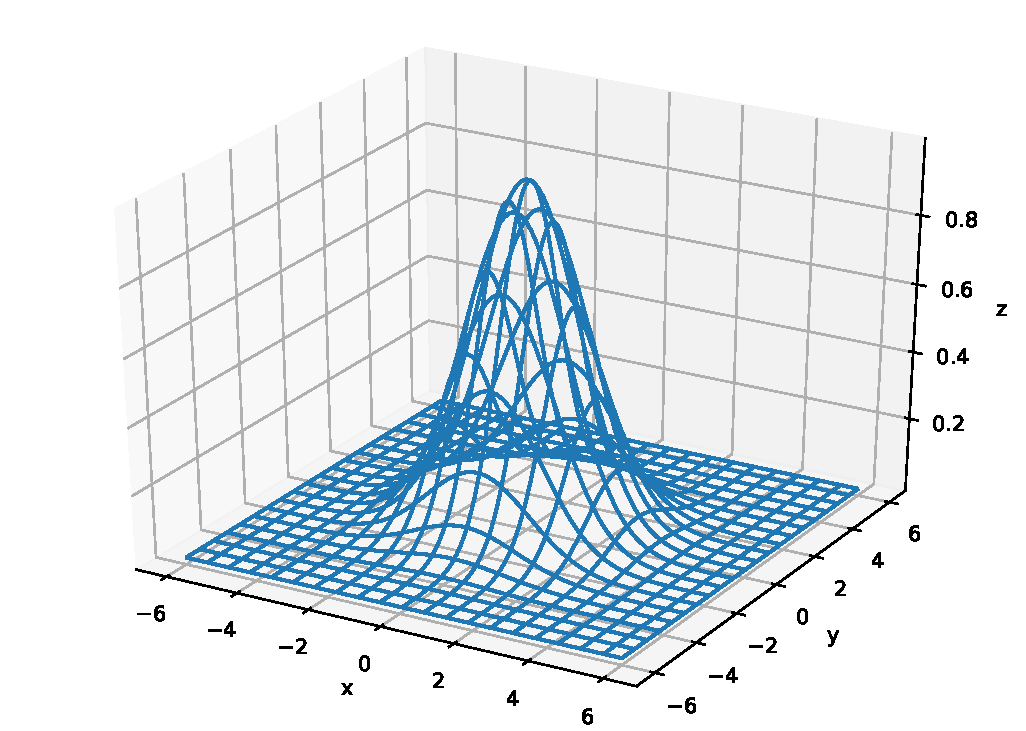
\includegraphics[width = 0.7\textwidth]{./figures/psf1.pdf}
	\caption{Exemplo de gráfico de uma função de espalhamento de ponto com $\gamma = 2$ centrada em $[0,0]$.}
	\label{fig:psfplot}
\end{figure}

\begin{figure}
	\centering
	
\includegraphics[width = 0.25\textwidth]{./figures/psfexample0.png}
	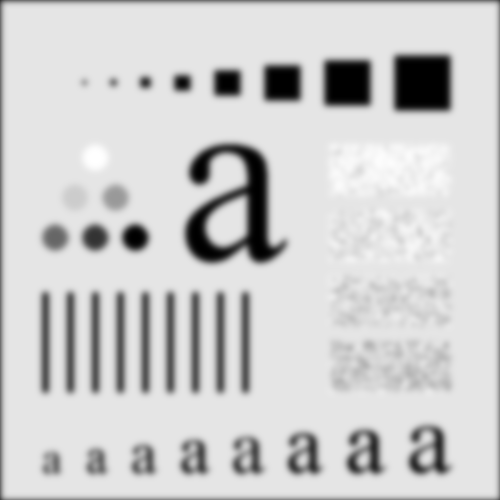
\includegraphics[width = 0.25\textwidth]{./figures/psfexample1.png}
	\caption{Exemplo de convolução de uma imagem com uma função de espalhamento de ponto com $\gamma = 10$.}
	\label{fig:psfexample}
\end{figure}

\begin{equation}
	\label{eq:psfcenter}
	\mathbf{u}^{(k)}_j = \mathbf{R}^{(k)}(\mathbf{v}_j-\mathbf{\overline{v}})+\mathbf{\overline{v}}+\mathbf{s}_k
\end{equation}

\begin{equation}
	\mathbf{R}^{(k)} = 
	\begin{pmatrix}
		\cos \theta_k & \sin \theta_k \\
		- \sin \theta_k & \cos \theta_k
	\end{pmatrix}
\end{equation}

\begin{figure}
	\centering
	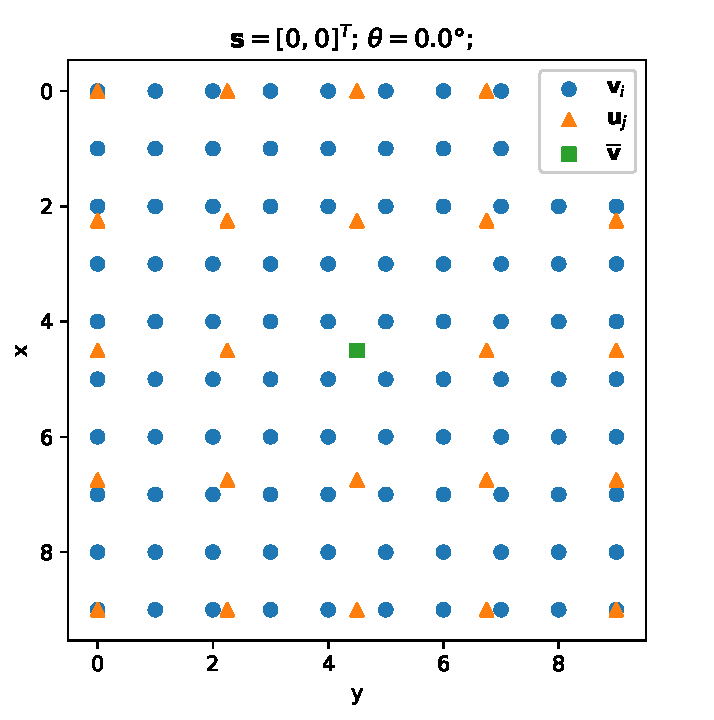
\includegraphics[width=0.3\textwidth]{./figures/transform1.pdf}
	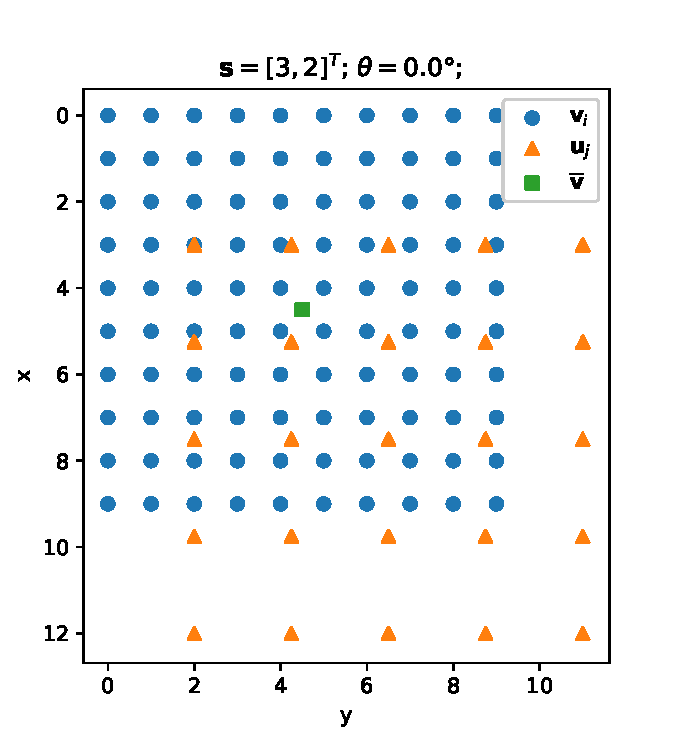
\includegraphics[width=0.3\textwidth]{./figures/transform2.pdf}
	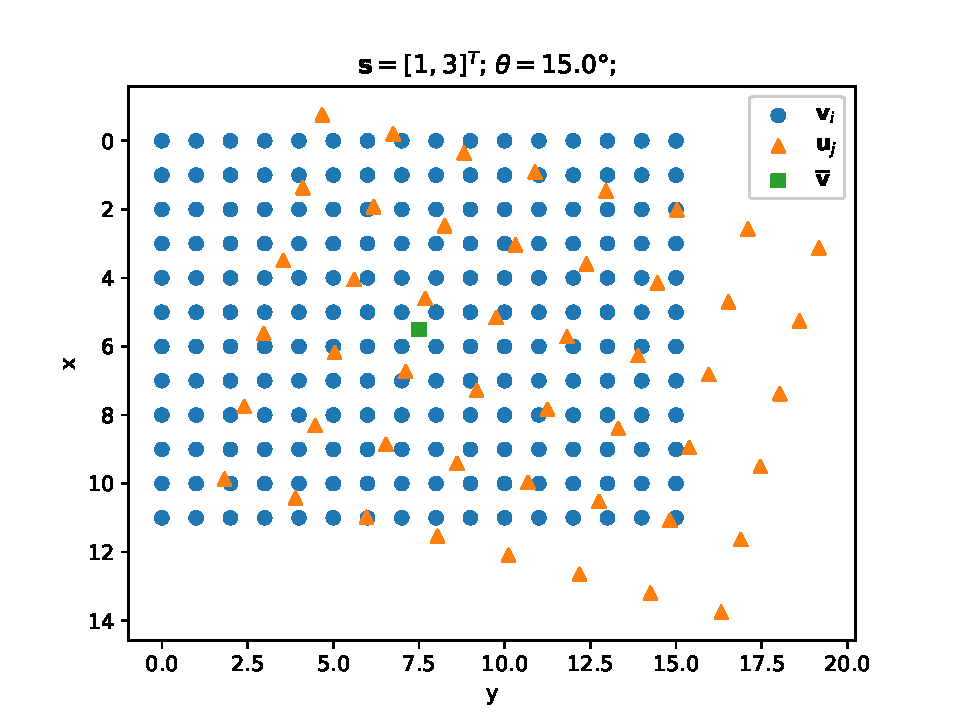
\includegraphics[width=0.3\textwidth]{./figures/transform3.pdf}
	\caption{Visualização das transformações de subamostragem, deslocamento linear e rotação.}
	\label{fig:transformations}
\end{figure}



\section{\label{sec:srmetodos}Apreciação dos Métodos de Super-resolução} 
Esta seção descreve resumidamente alguns dos métodos de super-resolução mais importantes 

A maioria dos algorítmos de super-resolução desenvolvidos faz o processamento de imagem no domínio espacial.
Os tipos de abordagens usadas são bastante diversos, sendo que a mais frequente é a probabilística, na qual o método usado neste trabalho está incluído \cite{nasrollahi2014super}.
\subsection{Métodos no domínio da frequência.}
Os primeiros algorítimos de super-resolução desenvolvidos faziam o processamento das imagens no domínio da frequência.
Esse tipo de abordagem tinha a vantagem da simplicidade em sua teoria.
No entanto, as técnicas de super-resolução no domínio da frequência tinham limitações com respeito ao tipo de degradação sofrida pela imagem além da dificuldade de aplicar o conhecimento a priori da imagem de alta resolução no domínio espacial para regularização.
Por estes e outros motivos que a maioria dos algorítimos de super-resolução desenvolvidos até hoje faz o processamento das imagens no domínio espacial \cite{park2003super}.

Os trabalhos de Gerchberg \cite{Gerchberg1974} e Santis e Gori \cite{de1975iterative} foram os primeiros a introduzir técnicas de super-resolução no domínio da frequência.
Sendo que o primeiro método a ter múltiplas imagens como entrada foi desenvolvido por Tsai e Huang em 1994 \cite{nasrollahi2014super}.
Este algorítimo foi desenvolvido para processar as imagens geradas pelo satélite Landsat 4.
Este satélite gerava várias imagens semelhantes, porém deslocadas, da mesma área na
terra.

Podemos considerar que cada imagem $g_k$ gerada pelo satélite seja uma versão deslocada de uma cena contínua $f$, podemos considerar que

\begin{equation}
	g_k(m,n) = f(m + \Delta_{m_k}, n + \Delta_{n_k}).
\end{equation}

Pela propriedade de deslocamento da transformada de Fourier, a transformada de Fourier contínua das imagens geradas pelo satélite, em relação à pode ser dada por

\begin{equation}
	F_{g_k} (m,n) = \exp{[i2\pi (\Delta_{m_k}m + \Delta_{n_k}n)]} F_f (m,n).
\end{equation}

Tendo isso, a transformada discreta de Fourier de $g_k$ é dada por

\begin{equation}
	G_k(m,n) = \frac{1}{T_m T_n} \sum^\infty_{p_1=-\infty} \sum^\infty_{p_2=-\infty}
	F_{g_k} \left( \frac{m}{MT_m} + p_1 \frac{1}{T_m},
	\frac{n}{NT_n} + p_2\frac{1}{T_n} \right).
\end{equation}

Segundo Nasrollahi e Moeslund \cite{nasrollahi2014super} o problema de super-resolução se resolve encontrando a transformada contínua de Fourier ($\mathbf{F_f}$) que soluciona (\ref{eq:dft_tsai}).
Isso pode ser resolvido usando o Método dos Mínimos Quadrados.

\begin{equation}
	\label{eq:dft_tsai}
	\mathbf{G} = \mathbf{\Phi F_f}
\end{equation}

% ISSUE: Completar seção domínio da frequência.




\subsection{Iterative Back Projections}
% ISSUE: Tentar mudar a formatação de subsubsection

O método \emph{Iterative Back Projection} ou retroprojeção iterativa (tradução do autor) foi proposto pela primeira vez por Irani e Peleg \cite{irani1991improv}.
Trata-se de um método iterativo que visa minimizar o erro a cada execução.

% ISSUE: Inserir IBP na lista de siglas.

A cada interação do método IBP, uma imagem de alta resolução é estimada.
Então é usado o modelo de observação para gerar um conjunto simulado de imagens de baixa resolução.
Esse conjunto de imagens simuladas é comparado às imagens de baixa resolução obtidas através do sistema de aquisição.
A comparação se dá através do cálculo da diferença (erro) entre os dois conjuntos de imagem.
O método iterativo busca minimizar esse erro afim de recuperar a imagem de alta resolução \cite{park2003super,reis2014metodo}.

% SUGGESTION: Inserir figura do esquema de IBP.
% SUGGESTION: Inserir equaçõ do algoritmo de IBP.

\subsection{Métodos de Aprendizado}
Os métodos de super-resolução baseados em aprendizado usam redes neurais para restaurar imagens estáticas.
Para que isso seja possível, deve haver uma etapa de aprendizado onde exemplos de imagens de uma classe específica (impressões digitais, rostos, texto) são usados junto com seus equivalentes de baixa resolução para que o algorítimo reconheça o relacionamento entre elas.
Esse conhecimento forma a componente a priori na reconstrução das imagens.

\subsection{Métodos Probabilísticos}
Os métodos probabilísticos se concentram em duas abordagens principais, a saber: máxima verossimilhança e máximo a posteriori \cite{nasrollahi2014super}.
Em resumo, os métodos de máxima verossimilhança estabelecem uma função de verossimilhança das imagens observadas baseada nos modelos de observação e no ruído


\chapter{Super Resolução Bayesiana}
\label{chap:srbayes}
\section{Introdução}
O método de super resolução desenvolvido no trabalho de Tipping e Bishop \cite{tipping2003bayesian} é um método probabilístico para a obtenção de uma imagem de alta resolução
a partir de um conjunto de imagens de baixa resolução de uma mesma cena.
Esse conjunto de imagens de baixa resolução poderiam ser retirados de quadros de um
vídeo produzido por uma câmera de segurança que fica parada em relação ao objeto
observado, por exemplo.

Pode-se dizer que a abordagem usada neste método é uma expansão do método de máxima
verossimilhança descrito na Seção \ref{sec:metodosprob}.
O método de super-resolução Bayesiana adiciona uma densidade de probabilidade como
conhecimento a priori da imagem para restringir a quantidade de soluções possíveis do
problema, contornando assim uma das inconveniências da abordagem de máxima verossimilhança.
A adição de uma densidade de probabilidade \emph{a priori}, converte a abordagem de máxima verossimilhança em uma abordagem de máximo \emph{a posteriori} (MAP).

% ISSUE: Adicionar resumo do capítulo de Super-resolução Bayesiana
% ISSUE: Excluir os parágrafos abaixo
se vale do método de inferência Bayesiana para obter uma imagem de alta resolução a partir de várias imagens de baixa resolução.
Através de um método de inferência Bayesiana, é possível obter uma estimativa de valores desconhecidos (como a imagem de alta resolução) usando um conhecimento a priori que se tem desses dados e informações que já estão disponíveis(no caso, as imagens de baixa resolução) \cite{therrien2011probability}.

Sabendo disso, há a necessidade de formular uma distribuição a priori que represente as características estatísticas da imagem que pretendemos estimar a partir dos dados.
A distribuição de probabilidade a priori escolhida para a imagem é uma gaussiana como descrita a seguir:

\section{Equacionamento do Método de Super-resolução Bayesiana}
A distribuição de probabilidade \emph{a priori} $p(\mathbf{x})$ é uma Gaussiana de média $\mathbf{0}$ e matriz de covariância $\mathbf{Z}_x$. A função que gera a matriz de covariância da distribuição \emph{a priori} da imagem é descrita em (\ref{eq:covmat}).

\begin{gather}
	\mathbf{x} \sim \mathcal{N}(\mathbf{0}, \mathbf{Z}_x) \\ 
	\label{eq:covmat} Z_x(i,j) = A \exp \left\{ - \frac{\|\mathbf{v}_i - \mathbf{v}_j \|^2}{r^2} \right\}
\end{gather}

Onde $A$ é uma constante escalar que indica a \emph{força} da distribuição e $r$ determina o quanto cada ponto da imagem de alta resolução depende dos pontos vizinhos.
Expandindo a função densidade de probabilidade $p(\mathbf{x})$ temos:

\begin{equation}
	\label{eq:priordist}
	p(\mathbf{x}) = \frac{1}{\sqrt{(2\pi)^N |\mathbf{Z}_x|}}\exp{-\tfrac{1}{2} \mathbf{x}^T \mathbf{Z}^{-1}_x \mathbf{x}}
\end{equation}

Este tipo de distribuição não é o ideal, visto que se definirmos $r=1$, estaríamos dizendo que a maioria dos valores dos pontos da imagem de de alta resolução estão contidos no intervalo $[-1,1]$, o que não condiz com a realidade do que se espera de uma imagem digital.
No entanto, o uso desta distribuição a priori será mantido no desenvolvimento deste
trabalho pela conveniência proporcionada pela função de probabilidade Gaussiana, que
facilita algumas manipulações -- como aplicação de logaritmos naturais e as marginalizações --  utilizadas a seguir.

Com base no modelo de observação em \ref{eq:degradation} e no que foi descrito na Seção \ref{sec:metodosprob}, a distribuição de probabilidade de $\mathbf{y}^{(k)}$ condicionada uma estimativa dos parâmetros e da imagem de alta resolução é dada por:

\begin{equation}
	\label{eq:likelihood0}
	p(\mathbf{y}^{(k)} | \mathbf{x}, \mathbf{s}_k, \theta_k, \gamma) = 
	\left(\frac{\beta}{2\pi}\right)^{M/2}
	\exp \left\{ -\frac{\beta}{2} \| \mathbf{y}^{(k)} - \mathbf{W}^{(k)} \mathbf{x} \|^2 \right\}.
\end{equation}

% Note que esta distribuição é condicionada na imagem de alta resolução e nos parâmetros de degradação, dados que são desconhecidos em um situação real.

A proposta de Super-resolução Bayesiana é usar o teorema de Bayes para obter uma função
de probabilidade \emph{a posteriori} da imagem $\mathbf{x}$; ou seja, uma função de
probabilidade que resulte da aplicação de um conhecimento \emph{a priori} da imagem à
abordagem de máxima verossimilhança. A Equação \ref{eq:posteriordist} mostra como foi aplicado o Teorema de Bayes para obter uma função de probabilidade \emph{a posteriori} da imagem.

\begin{equation}
	\label{eq:posteriordist}
	p(\mathbf{x}|\{\mathbf{y}^{(k)},\mathbf{s}_k,\theta_k\}, \gamma) = 
	\frac{p(\mathbf{x})\prod^K_{k=1} p(\mathbf{y}^{(k)}|\mathbf{x},\mathbf{s}_k,\theta_k, \gamma)}
	{p(\{\mathbf{y}^{(k)}\}|\{\mathbf{s}_k,\mathbf{\theta}_k\},\gamma)} \\
\end{equation}


Esclarecendo que $\{\mathbf{y}^{(k)}\}$ é o conjunto de todos $\mathbf{y}^{(k)}$ para $k = 1,2,...,K$.
Esta lógica também se aplica aos conjuntos $\{\mathbf{s}_k,\mathbf{\theta}_k\}$.

Esta função de probabilidade já poderia ser utilizada para inferir a imagem de alta resolução.
Para isso, bastaria encontrar o valor de $\mathbf{x}$ que maximiza o numerador em (\ref{eq:posteriordist}). entretanto, isso exigiria saber os valores dos parâmetros de degradação ($\gamma$, $\theta_k$, $\mathbf{\theta}_k$).
Como esses parâmetros não estão disponíveis, eles também terão de ser estimados a partir das imagens de baixa resolução $\mathbf{y}_k$. 
Algumas abordagens procuram otimizar os parâmetros de degradação concomitantemente com a imagem usando a distribuição em (\ref{eq:posteriordist}) (ao que o trabalho de Tipping \cite{tipping2003bayesian} se refere como "abordagem MAP"). No entanto, esta abordagem não leva em consideração a incerteza ao determinar a imagem de alta resolução e as consequências disso na estimação dos parâmetros.

Os parâmetros de degradação $\mathbf{s}_k$, $\theta_k$ e $\gamma$ devem ser estimados a partir de uma distribuição marginal que, segundo Pickup \cite{pickup2007bayesian2}, é dada por:

\begin{equation}
	\label{eq:marginalization}
	p(\{\mathbf{y}^{(k)}\} | \{\mathbf{s}_k, \theta_k \}, \gamma) = 
	\int  p(\mathbf{x})\prod^K_{k=1} p(\mathbf{y}^{(k)}|\mathbf{x},\mathbf{s}_k,\theta_k, \gamma) \mathrm{d}\mathbf{x}.
\end{equation}

Fazendo as devidas aplicações de (\ref{eq:likelihood0}) e (\ref{eq:priordist}), a expressão em (\ref{eq:marginalization}) se avalia como uma distribuição Gaussiana de $\{\mathbf{y}^{(k)}\}$ na forma
\begin{equation}
	\mathrm{y} \sim \mathcal{N}(\mathbf{0}, \mathbf{Z}_y)
\end{equation}
onde $\mathrm{y}$ é um vetor empilhado de todas as imagens de baixa resolução e
\begin{equation}
	\mathbf{Z}_y = \beta^{-1} \mathbf{I} + \mathrm{W} \mathbf{Z}_x \mathrm{W}^T.
\end{equation}


Condensando tudo e fazendo as devidas manipulações de matrizes, obtemos a função de verossimilhança em (\ref{eq:parameter}), onde foi aplicado o logaritmo e descartados os termos que não dependem dos parâmetros de degradação.

\begin{gather}
	\label{eq:parameter}
	\log p(\mathrm{y}|\{\mathbf{s}_k,\theta_k\}, \gamma) = -\frac{1}{2}\left[\beta \sum^K_{k=1} \|\mathbf{y}^{(k)} - \mathbf{W}^{(k)}\boldsymbol{\mu}\|^2
    + \boldsymbol{\mu}^T\mathbf{Z}_x \boldsymbol{\mu}
    \vphantom{\int_t} + \log |\mathbf{Z}_x| - \log{|\Sigma |} \right] \\
%	= \mathcal{N}(\boldsymbol{\mu},\mathbf{\Sigma}) \\
	\mathbf{ \Sigma }= \left[\mathbf{Z}^{-1}_x + \beta \left( \sum^K_{k = 1} \mathbf{W}^{(k)^T} \mathbf{W}^{(k)} \right) \right]^{-1} \\
	\boldsymbol{\mu} = \beta \mathbf{ \Sigma } \left( \sum^K_{k=1} \mathbf{W}^{(k)^T}\mathbf{y}^{(k)} \right).
\end{gather}

Em uma situação ideal, a melhor estimativa dos valores dos parâmetros de degradação é a que maximiza a função de verossimilhança em (\ref{eq:parameter}).
Tendo a estimativa desses valores, podemos então usá-los em (\ref{eq:posteriordist}) para procurar pela imagem de alta resolução $\mathbf{x}$ que maximiza aquela distribuição de probabilidade.

Um fato que se constatou empiricamente na tentativa de calcular os valores da função de verossimilhança é que as probabilidades são muito pequenas ao ponto de estarem fora do intervalo de precisão de uma variável do tipo ponto flutuante.
Os valores também variam muito pouco ao longo do espaço vetorial de $\mathbf{x}$ o que dificultaria o uso de métodos iterativos para encontrar o ponto de máximo da função.


Para resolver isso, aplicou-se o logaritmo natural à função. Isso resolveu o problema da escala e da variação.
Além disso eliminou os exponenciais e os produtos, facilitando o cálculo do gradiente, necessário na aplicação dos algorítimos de otimização.

\begin{gather}
	\label{eq:imageLikelihood} \mathcal{L}(\mathbf{x}) = -\frac{1}{2} \left\{ \sum^K_{k=1} \|\mathbf{y}^{(k)} - \mathbf{W}^{(k)} \mathbf{x} \|^2 + \mathbf{x}^T\mathbf{Z}^{-1}_x\mathbf{x} - KM\log{(\beta)} - \log{|\mathbf{Z}_x|} \right\} \\ 
	\label{eq:imageLikelihood_gradient} \mathcal{L}'(\mathbf{x}) =  \sum^K_{k=1}  (\mathbf{y}^{(k)} - \mathbf{W}^{(k)}\mathbf{x})(\mathbf{W}^{(k)})^T  - \frac{1}{2}(\mathbf{Z}^{-1}_x + (\mathbf{Z}^{-1}_x)^T)\mathbf{x}  
	% L''(\mathbf{x}) =  -\sum^K_{k=1} (\mathbf{W}^{(k)})^T\mathbf{W}^{(k)} - \frac{1}{2}(\mathbf{Z}^{-1}_x - (\mathbf{Z}^{-1}_x)^T)^T
\end{gather}

Com tudo isso, já temos todas as ferramentas necessárias para estimar os parâmetros de degradação e usá-los para inferir a imagem de alta resolução.
Tanto a função em (\ref{eq:imageLikelihood}) quanto a função de probabilidade \emph{a posteriori} podem ser otimizadas usando métodos iterativos.
Isso será melhor discutido no Capítulo \ref{chap:resultados}.


\chapter{Resultados}
\label{chap:resultados}
\section{Introdução}
Para avaliar a eficácia do método de super-resolução bayesiana, 
foi elaborado um teste que simula um sistema de aquisição de imagem,
gerando as imagens de baixa resolução a serem restauradas.
Na sequência, as imagens de baixa resolução foram submetidas ao método de super-resolução como descrito capítulo \ref{chap:srbayes}.

Este capítulo descreve o processo de implementação e teste do método de super-resolução bayesiana.
A seção \ref{sec:gerimagens} apresenta o processo que gerou as imagens de teste simulando as transformações aplicadas pelo sistema de aquisição.
A seção \ref{sec:parestimation} relata como se deu o processo de restauração da imagem de alta resolução a partir do conjunto de imagens de baixa resolução.

\section{Geração do conjunto de imagens de teste}
\label{sec:gerimagens}
As imagens usadas para testar o método de restauração descrito neste trabalho foram geradas artificialmente a partir de uma única imagem usando o modelo de observação descrito na seção \ref{sec:obsmodel}.
Para os testes reportados aqui foi usada a imagem da Figura \ref{fig:hrimage}.
Usando o modelo de observação, foram geradas 20 imagens de baixa resolução como as da Figura \ref{fig:frames}.
Para diminuir o custo computacional do processo, a imagem foi convertida para escala de cinza antes da degradação.

\begin{figure}[h]
	\centering
	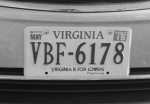
\includegraphics{figures/imtestes.png}
	\caption{Imagem de alta resolução utilizada nos testes.}
	\label{fig:hrimage}

\end{figure}

Para os testes feitos neste trabalho, a imagem de alta resolução foi reamostrada de forma que as dimensões das imagens de baixa resolução são iguais a $0.25$ vezes as dimensões da imagem HR.  
Dessa forma, há 16 pontos na imagem de alta resolução para cada ponto na imagem de baix resolução.
A largura da função de espalhamento de ponto ($\gamma$) escolhida foi 2.
Para cada imagem, o ângulo de rotação foi escolhido aleatoriamente de uma distribuição uniforme entre $-4$ e $4$ graus.
A mesma seleção aleatória foi feita para o deslocamento linear da imagem; a quantidade de pontos de deslocamento foi retirada de uma distribuição uniforme e contínua entre $-2$ e $2$ em cada um dos eixos.
A tabela \ref{tab:resumoParametros} resume os parâmetros utilizados na degradação das imagens.

\begin{figure}[H]
	\centering
	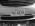
\includegraphics{figures/degradedImg/result-0.png}
	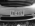
\includegraphics{figures/degradedImg/result-1.png}
	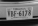
\includegraphics{figures/degradedImg/result-2.png}
	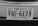
\includegraphics{figures/degradedImg/result-3.png}
	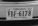
\includegraphics{figures/degradedImg/result-4.png}
	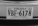
\includegraphics{figures/degradedImg/result-5.png}
	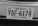
\includegraphics{figures/degradedImg/result-6.png}
	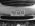
\includegraphics{figures/degradedImg/result-7.png}
	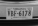
\includegraphics{figures/degradedImg/result-8.png}
	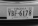
\includegraphics{figures/degradedImg/result-9.png} \\
	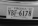
\includegraphics{figures/degradedImg/result-10.png}
	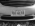
\includegraphics{figures/degradedImg/result-11.png}
	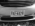
\includegraphics{figures/degradedImg/result-12.png}
	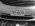
\includegraphics{figures/degradedImg/result-13.png}
	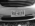
\includegraphics{figures/degradedImg/result-14.png}
	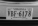
\includegraphics{figures/degradedImg/result-15.png}
	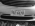
\includegraphics{figures/degradedImg/result-16.png}
	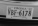
\includegraphics{figures/degradedImg/result-17.png}
	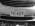
\includegraphics{figures/degradedImg/result-18.png}
	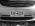
\includegraphics{figures/degradedImg/result-19.png}
	\caption{Conjunto das imagens geradas a partir da imagem de alta resolução. A diferença sutil entre as imagens é causada pelas transformações de deslocamento e rotação.}
	\label{fig:frames}
\end{figure}

\begin{table}[h]
	\centering
	\caption{Parâmetros de degradação usados para gerar o conjunto de imagens de teste.}
	\label{tab:resumoParametros}
	\begin{tabular}{r | l}
		Ângulos de rotação ($\theta_k$) & $ \sim \mathcal{U}(-4, 4)$ \\ \hline
		Deslocamento ($\mathbf{s}_k$)& $\sim \mathcal{U}(-2,2)$\\ \hline
		Largura da PSF ($\gamma$) & 2 \\ \hline
		Dimensões da imagem de alta resolução & $139 \times 104$ \\ \hline
		Dimensões das imagens de baixa resolução & $35 \times 26$ \\

	\end{tabular}
\end{table}

O processo de geração das imagens de baixa resolução foi todo desenvolvido usando a linguagem Python,
beneficiando-se dos módulos Numpy e Pillow.
Os parâmetros de degradação bem como as dimensões da imagem original foram salvas em arquivos de valores separados por vírgula (csv) junto com as imagens geradas.
Isso foi necessário para que fosse possível validar os resultados das etapas de restauração.

\section{Estimação dos parâmetros de degradação}
\label{sec:parestimation}
A primeira etapa no processo de restauração da imagem é estimar os parâmetros que definiram as transformações que degradaram a imagem durante o processo simulado de captura.Como já elucidado no capítulo \ref{chap:srbayes}, encontrar os valores dos parâmetros de degradação é um problema de otimização.
Teoricamente, os valores verdadeiros de $\mathbf{s}_k$, $\theta_k$ e $\gamma$ são os que maximizam a função de verosimilhança em \ref{eq:parameter}.

O artigo no qual este trabalho se baseia relata que o método de otimização usado
para estimar tanto os parâmetros de degradação quanto a imagem foi o de gradientes
conjugados \cite{tipping2003bayesian}.
Como o método de super-resolução deste trabalho foi todo escrito em Python,
não foi possível utilizar o mesmo método de implementação utilizado no artigo.
Em vez disso, foi usado um Método de Newton Truncado presente no módulo \emph{Scipy}.

% SUGGESTION: Falar mais sobre o algorítimo de otimização Método de Newton Truncado.
% NOTE: Talvez esta seção mude se for feita otimização de gamma.

O processo de otimização dos parâmetros se deu da seguinte forma:
Os parâmetros iniciais foram definidos como zero.
Primeiramente, somente os valores de deslocamento são otimizados enquanto os valores dos ângulos de rotação ficam fixos.
Só após isso que é realizada a otimização dos ângulos de rotação junto com os deslocamentos lineares.
Essa abordagem é usada no artigo original e os testes realizados para este trabalho
constataram que a otimização dos parâmetros de deslocamento se aproxima mais rápido da
solução correta quando esses valores são estimados isoladamente.
A estimação dos ângulos também funciona melhor quando os valores de deslocamento já estão
otimizados.



Como a função em \ref{eq:parameter} não é uma função vetorial do tipo $ f(\mathbf{x}) : \mathbb{R}^n \to \mathbb{R}^1 $.
Por isso, a função de verossimilhança foi empacotada de forma que receba todos os parâmetros de entrada na forma de um vetor e retorne somente um escalar na saída.

Em vez de otimizar todos os parâmetros ao mesmo tempo,
constatou-se que a otimização converge mais rápido se os valores 

\section{Estimação da imagem de alta resolução}
% ISSUE: Seção de estimação da imagem

\chapter{Conclusão}
% RESUMO DO QUE FOI FEITO
Este trabalho apresentou a teoria e relatou a implementação e os resultados do desenvolvimento de um método de Super-Resolução Bayesiana aplicado na restauração de imagens de placas de veículos.

As principais características do método proposto são:
\begin{itemize}
	\item Obtêm uma imagem de alta resolução a partir de um conjunto de imagens de baixa resolução.
	\item Incorpora uma distribuição de probabilidade como conhecimento \emph{a priori} acerca da imagem de alta resolução.
	\item Usa um método de inferência Bayesiana para estimar os parâmetros de degradação e a imagem de alta resolução em si.
	\item O uso de um método iterativo de otimização baseado e gradiente para estimar tanto os parâmetros de degradação quanto a própria imagem.

\end{itemize}

% AVALIAÇÃO
A etapa de estimação dos parâmetros de degradação obteve resultados com precisão adequada considerando o custo em tempo computacional.
A estimação dos ângulos e dos deslocamentos foi capaz de diminuir o erro em relação aos parâmetros verdadeiros.
No entanto, o modelo proposto não foi eficaz em estimar a largura da função de espalhamento de ponto com a mesma precisão.

Em uma análise subjetiva, a aplicação do método de Super-Resolução Bayesiana obteve resultados satisfatórios. 
Como é possível observar na Figura \ref{fig:results_compare}, o método de super-resolução obteve resultados qualitativamente melhores do que um método mais simples como uma interpolação. Isso se deve ao fato de que o método de super resolução é capaz de recuperar as componentes de alta resolução da imagem que se perdem durante o processo de captura.

% TRABALHOS FUTUROS
Como propostas para trabalhos futuros podemos citar: a aplicação do método à imagens
coloridas, visto que a única mudança seria na etapa de estimação da imagem,
quando o algorítmo de otimização deve ser aplicado aos três canais da imagem;
a redução do custo computacional do algoritmo, sobretudo a etapa de estimação da imagem
que depende de matrizes com mais de 15000 elementos.

% ISSUE: Falar de pelo menos mais uma proposta de trabalho futuro.


% ELEMENTOS PÓS-TEXTUAIS
\postextual

% Referências bibliográficas
\bibliographystyle{plain}
\bibliography{referencias}


\end{document}
